\documentclass[a4paper,10pt]{article}

% includes
\usepackage{authblk}
\usepackage[english]{babel}
\usepackage{fancyvrb}
\usepackage[margin=3cm]{geometry}
\usepackage{graphicx}
\usepackage{hyperref,cleveref}
\usepackage[utf8]{inputenc}
\usepackage{mathpazo}
\usepackage{parskip}
\usepackage{soul} % highlight text
\usepackage{xcolor}

% macros
\newcommand{\todo}[1]{\textcolor{red}{\hl{\textbf{ToDo}}}: #1} % TODO item
\newcommand{\link}[1]{\href{#1}{\textcolor{blue}{\texttt{#1}}}} % hyperlink
\newcommand{\docdb}[1]{\href{https://www.snolab.ca/snoplus/private/DocDB/cgi/ShowDocument?docid=#1}{DocDB-#1}} % DocDB item

% title page
\title{Commissioning the Sussex remote control room}
\author{Martti Nirkko, Michal Rigan}
\affil{University of Sussex}
\date{\today}

%%%%%%%%%%%%%%%%%%%%%%%%%%%%%%%%%%%%%%%%%%%%%%%%%%%%%%%%%%%%%%%%%%%%%%%%%%%%%%%%

% main matter
\begin{document}

\maketitle

\begin{abstract}
This document describes the recent commissioning of another remote shift station for SNO+, the Control Room at Sussex (CRSU). Three machines were set up following available instructions for commissioning remote control rooms, and a virtual machine was used to run the phone software. The network stability was monitored over the course of 7 days, followed by 3 days of shadow shifts from 20th -- 22nd April 2018. A number of problems were encountered, all of which were successfully debugged. First detector shifts were taken at CRSU from 11th -- 17th May (Michal) and 28th -- 31st May (Martti). Some additional test were done regarding network stability and ORCA stability. The results of the commissioning, including testing and errors encountered are discussed in this document.
\end{abstract}

%%%%%%%%%%%%%%%%%%%%%%%%%%%%%%%%%%%%%%%%%%%%%%%%%%%%%%%%%%%%%%%%%%%%%%%%%%%%%%%%

\section{The Sussex control room}
The remote shift station was set up in the ``InvisiblesLab'' (4A23), a laboratory used by Simon Peeters' group located in Pevensey II building, right next to the SNO+ group members' offices. To enter the lab, the shifter must know the 4-digit door code. To obtain the code, the lab's safety briefing must have been completed. To gain entry to the building outside normal office hours, the shifter must acquire a SALTO access card from the MPS school offices. Note that the access card needs to be used regularly (every 3 months) in order to stay valid, which turned out to be a problem for one of the shifters. Since a second shifter was already in the building at the time, this was not a huge issue. Once in the building, it is very easy to renew the access card as it does not require human interaction. This card is a standard for any postgraduate student and staff at the university.

\subsection{Hardware specifications}
The requirements for remote shift stations are outlined in \cite{doc4428}. The minimal requirements at the time of writing are 4 CPUs and 8~GB RAM both for the monitoring machine(s) running CentOS~6, and the Mac running OSX 10.13 (High Sierra). The recommended iMac was purchased, while available towers were used for the monitoring machines. The hardware specifications for all machines can be found in \Cref{specs}. Note that the macOS was upgraded to 10.13.4 prior to shadow shifting.

Additional peripherals (monitor, speakers etc.) were added on 25/05/2018, and an Uninterruptible Power Supply (UPS\footnote{Eaton 5P 1550VA UPS Uninterruptible Power Supply, 230V Output, 1.1kW, 10A, {\tt \href{https://uk.rs-online.com/web/p/ups-uninterruptible-power-supplies/8239391/}{https://uk.rs-online.com/}}}) was installed on 29/01/2019. The final setup is shown in \Cref{crsu_setup}.

\begin{table}[htp]
	\centering
	\caption{Hardware specs for the CRSU computers. Note that the monitoring machine also runs Windows 7 on a virtual machine (VM), to which 1 CPU core and 8~GB RAM are allocated.}
	\label{specs}
	\vspace{3mm}
	    \small
	\def\arraystretch{1.2} % less crammy
	\begin{tabular}{| l | l | l | l |}
		\hline
		& \textbf{Operating machine} & \textbf{Monitoring machine 1} & \textbf{Monitoring machine 2}\\ \hline
		Hostname & {\tt mps019491.phys.susx.ac.uk} & {\tt cssd018593.ad.susx.ac.uk} & {\tt monsu2} \\ \hline
		Hardware & iMac (Retina 5K, 27'', 2017) & Dell T7910 workstation & Dell Optiplex 790\\ \hline
		System & macOS 10.13.4 (High Sierra) & CentOS 6.9 & CentOS 6.9 \\ \hline
		Processor & Intel Core i5 & Intel Xeon E5-2667 v3 & Intel Core i7 2600 \\ \hline
		\#CPUs & 4 cores (3.4 GHz) & 8 (16 virt.) cores (3.2 GHz) & 4 (8 virt.) cores (3.4 GHz) \\ \hline
		Memory & 8 GB (DDR4, 2400 MHz) & 128 GB (PC4, 2400MHz) & 8 GB (DDR3, 1333 MHz)\\ \hline
		Graphics & Radeon Pro 570 (4 GB) & NVIDIA NVS 310 (512 MB) & AMD Radeon HD 5450 \\ \hline
		Disk & 1 TB & 1.5 TB (RAID) & 1 TB \\ \hline
	\end{tabular}
\end{table}

\begin{figure}[htp]
	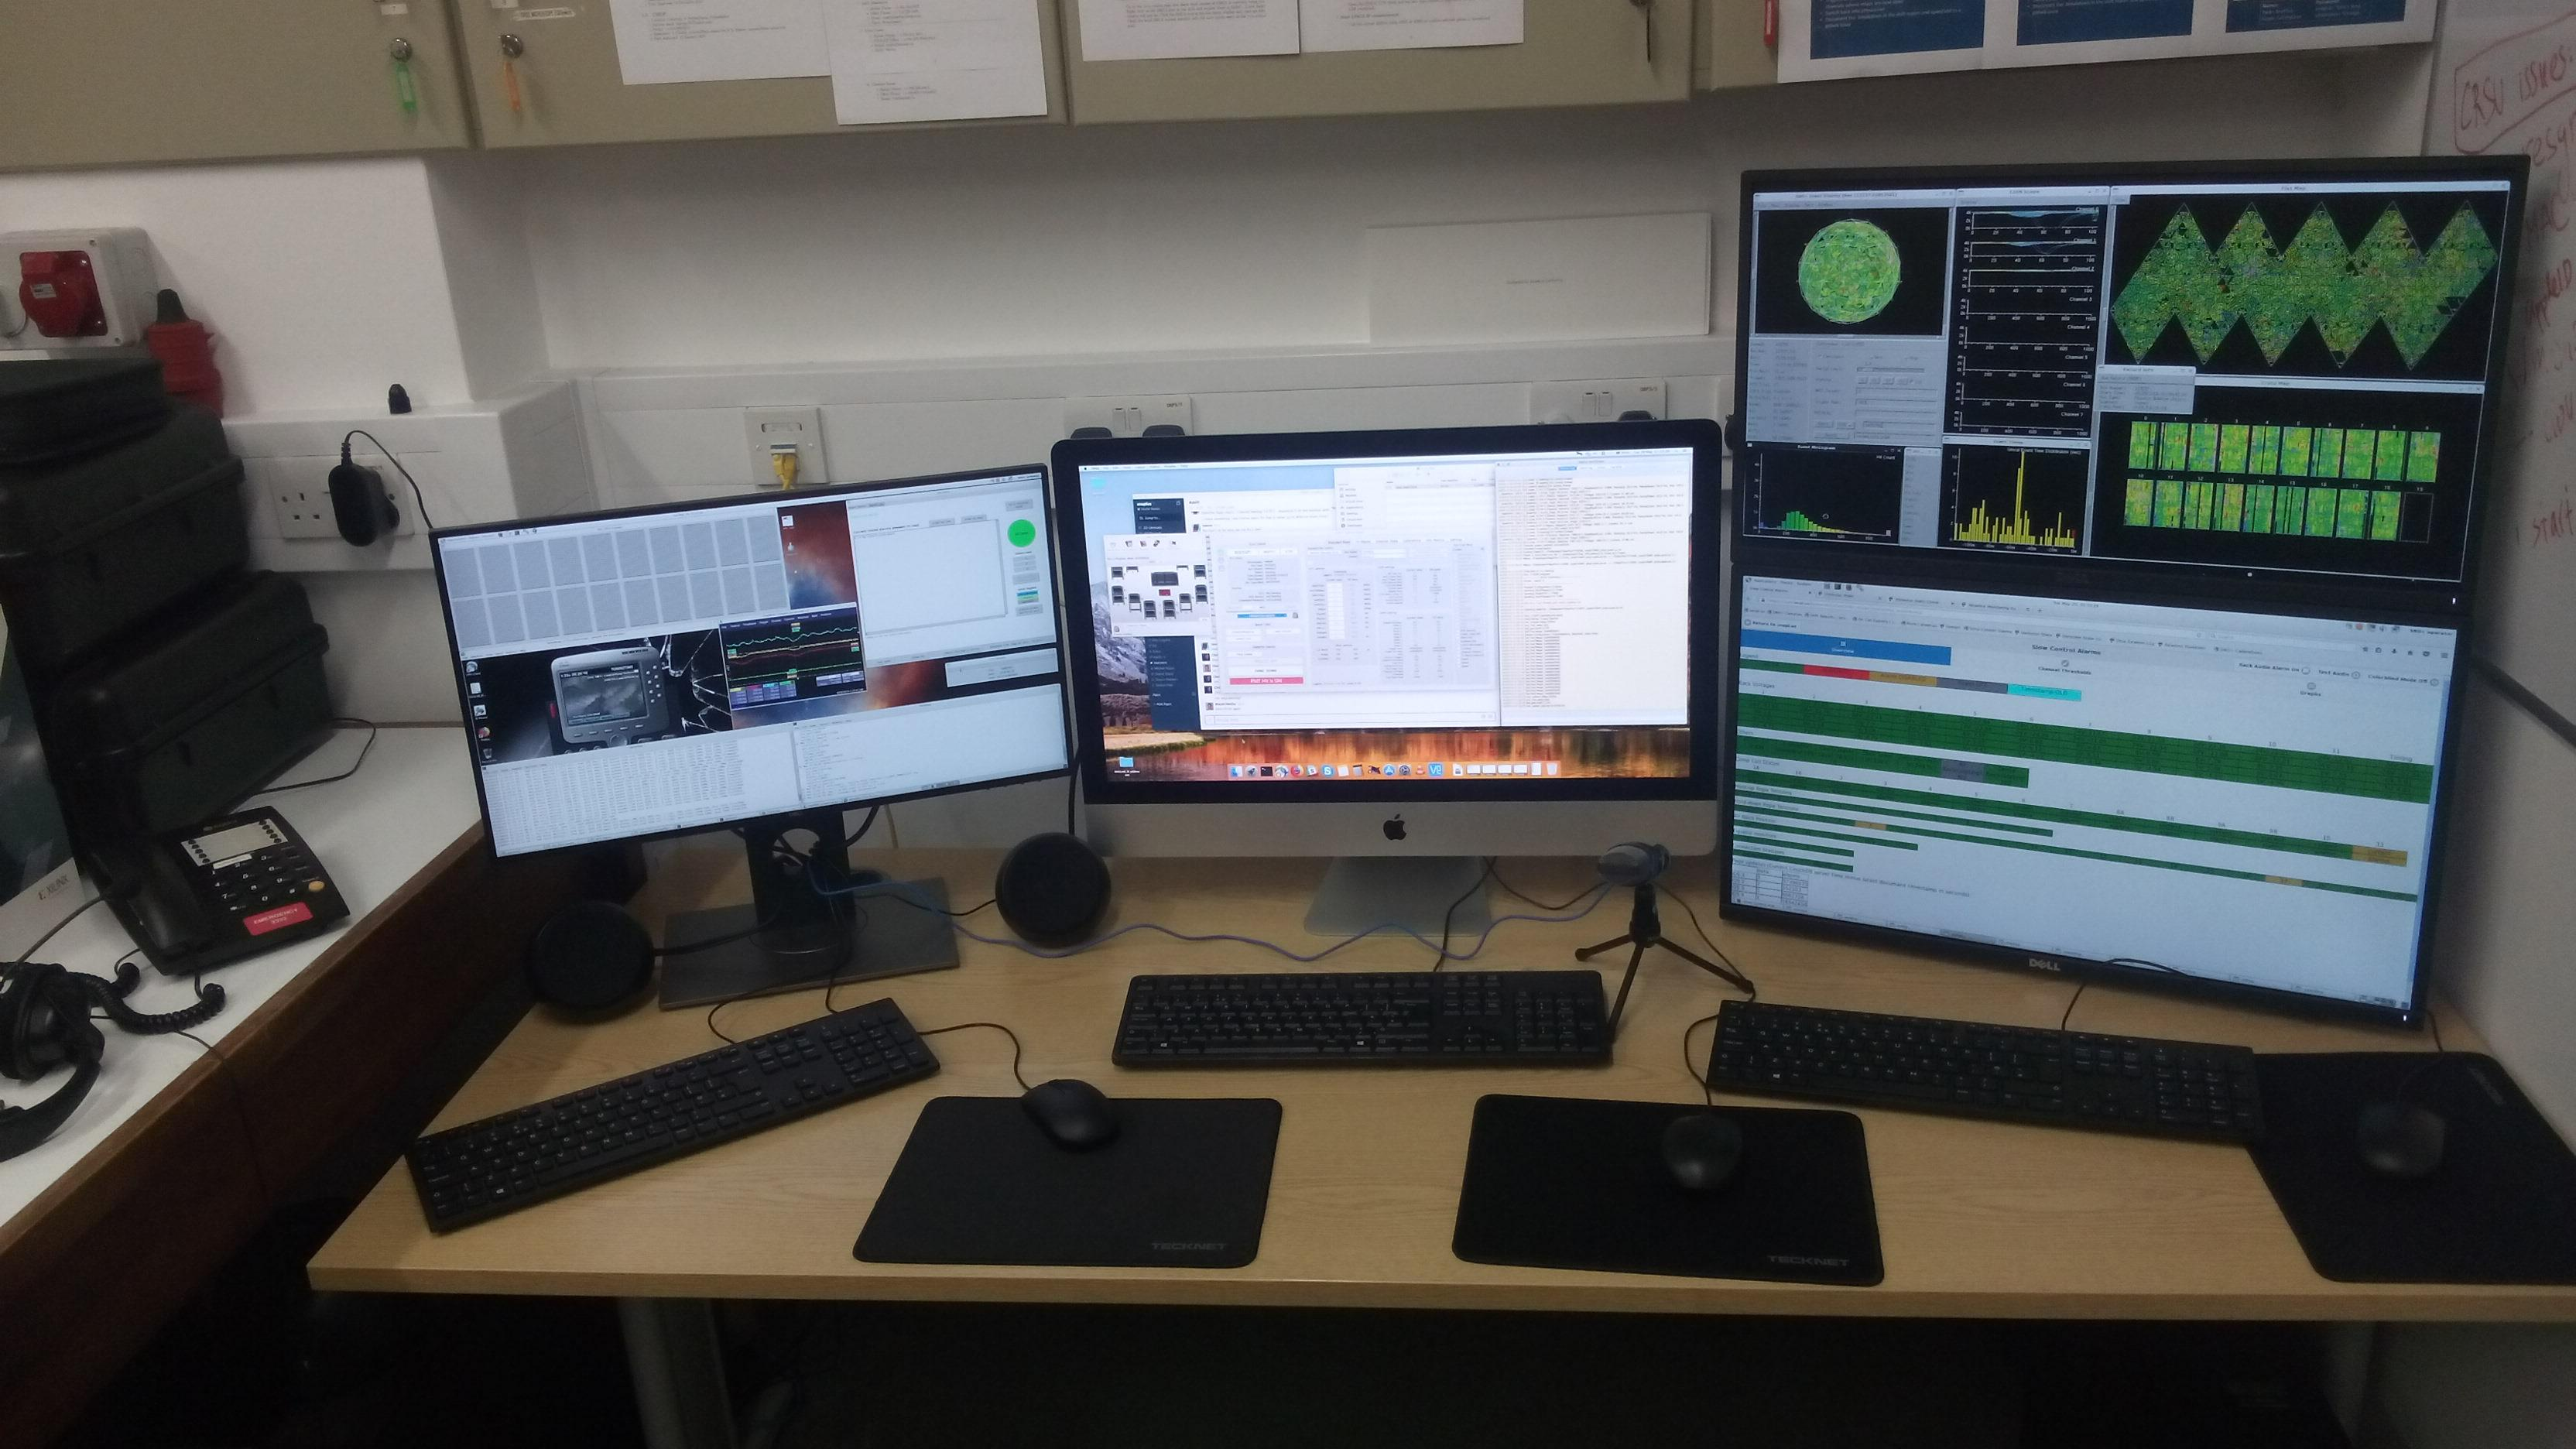
\includegraphics[width=\textwidth]{images/CRSU_final}
	\caption{Setup of the CRSU remote shift station. The screen on the left corresponds to monsu1, the iMac at the centre is opersu, and the two screens on the right are connected to monsu2. The landline telephone is located to the left of the screens. Additional peripherals include the 2.1 speaker system and the microphone, both of which are connected to monsu1. All devices except the landline phone (which is powered by an ethernet socket alone) are connected to the Uninterruptible Power Supply (UPS) at the bottom right.}
	\label{crsu_setup}
\end{figure}

\subsection{Installation}
The official remote control room procedures are outlined in \cite{doc4776}. The software was set up accordingly. It proved difficult to install CentOS on the large Dell tower (monsu1), as we decided to set up a dual-boot alongside the pre-installed Windows OS, in case that machine were to be used again for high-end graphics applications in the future. Additional graphics drivers also needed to be installed.

The installation of the Mac OS was done by ITS, to ensure a supported image of the operating system is used. This caused some problems when changing the system settings (e.g. timezone), as they kept reverting to the University-specific defaults (e.g. UK/London). The issues were eventually fixed by contacting ITS to add the required exceptions for the machine in question. The updated settings will remain consistent, and the config management system will keep them enforced. If any settings need to be changed in the future, this will need to be done by ITS.

\subsection{Software setup}
To install the phone software, a Windows~7 license was purchased, and the system was installed as a virtual machine (VM) on the Linux computer.

The usual {\tt snoperator} account was set up on all machines, including the Windows VM. The monitoring machines have an admin account named {\tt snotdaq} with the usual password, which is needed to update the monitoring tools. This account shows up as ``SNO+ expert'' on the login screen. The iMac was set up by Sussex ITS, who configured it so that Martti's and Michal's personal accounts have admin rights, with which the {\tt snotdaq} account was created. Note that updating ORCA does not require admin privileges -- these are required only for changing system settings, upgrading the OS, etc.

A number of desktop entries were created to start the builder log, trigger scope and supernova GUI on the monitoring machines, for instance:
{\small
\begin{Verbatim}[xleftmargin=-8mm]
	[Desktop Entry]
	Encoding=UTF-8
	Name=Builder
	Comment=Launch Builder
	Exec=ssh -t snoperator@buffer1.sp.snolab.ca 'tail\_log /raid/data/l1; exec bash -l'
	Icon=utilities-terminal
	Type=Application
	Terminal=true
\end{Verbatim}
}

%%%%%%%%%%%%%%%%%%%%%%%%%%%%%%%%%%%%%%%%%%%%%%%%%%%%%%%%%%%%%%%%%%%%%%%%%%%%%%%%

\section{Networking}

\subsection{VPN setup}
Each computer uses the Cisco Anyconnect Client recommended by SNOLAB. The user logs into the SNOLAB VPN using their personal account ({\tt SL-SNOPLUS} for operating and monitoring, {\tt SL-GEN} for the Windows VM). It is essential for the user to know their login before starting a shift! Anyone planning to do shifts should test this in advance by logging into the SNOLAB webmail service: 

\qquad\link{https://webmail.snolab.ca/}

Mac OSX has notoriously bad DNS resolution, i.e. it can't match hostnames to IP addresses. We found that the easiest solution is to manually map all the SNOLAB machines in the {\tt hosts} file, which fixed the problem. To get the hostnames, we used the Nagios webpage (go to ``Hosts''):

\qquad\link{https://snopl.us/nagios/}

To get the IP addresses, we used the {\tt getent} command (embedded in a loop), e.g.:
\begin{Verbatim}[xleftmargin=-8mm]
	$ getent hosts www.snolab.ca
	142.51.70.169   www.snolab.ca
\end{Verbatim}
This output can be copied as is to {\tt /etc/hosts} (requires {\tt sudo} rights).

\subsection{Connection stability}
In order to ensure a stable network connection, we contacted ITS to ensure connection stability. The network cabling between the PC and the switch were replaced, and all computers were moved to a different switch with very few occupied ports ($<25\%$). This has helped fix network performance issues in the past, according to ITS.

The network stability was tested over the course of 7 days on both machines using Karin's scripts described in \cite{doc5040}. These basically use the {\tt wget} command to ping the main Google/SNOLAB websites, for which the results were identical. A third script pings {\tt buffer1}, a machine only visible from within the SNOLAB VPN. A python script plots the results (we had to modify it a little due to locale changes, UK computers don't like the EDT timezone). No internet outages were registered, except when the ethernet cables were briefly unplugged to reroute the machines to a different switch. The VPN connection regularly fails to ping on-site machines, but the downtime is never more than 30 seconds. Note that such a ``reconnect'' is not logged as a ``disconnect'' by the Cisco VPN client (see statistics tab).

\subsection{Latency}
Because the above results are not very informative with regards to latency, we decided to continuously ping a machine on the VPN network. This was started 4~days before the first shadow shift, and ended near the end of the shift. The average latency was 110~ms with a minimum of 102~ms, although it regularly increased to up to 140~ms about once an hour (presumed to be caused by some increase in network activity on-site). Single events caused even higher spikes, but these were only temporary. The most significant increase occurred when we started shifting, with the latency fluctuating up to 200~ms with some even higher spikes.

It was during shifts that most of the latency-related problems (time-outs etc.) occurred. This caused a lot of problems affecting detector operations, and was found to be caused by network-intensive ``streaming'' applications (e.g. {\tt xsnoed}). Some tests were therefore run under load over the course of 30 minutes. \Cref{load_linux,load_mac} show the latency for both machines during this test phase. It appears that the current threshold for a timeout at 150~ms is still too low, and the problems observed overseas would be resolved by increasing it to 250~ms. The increase in latency was less extreme on the Mac, which only runs ORCA and the TUBii audio.

\begin{figure}[htp]
	\centering
	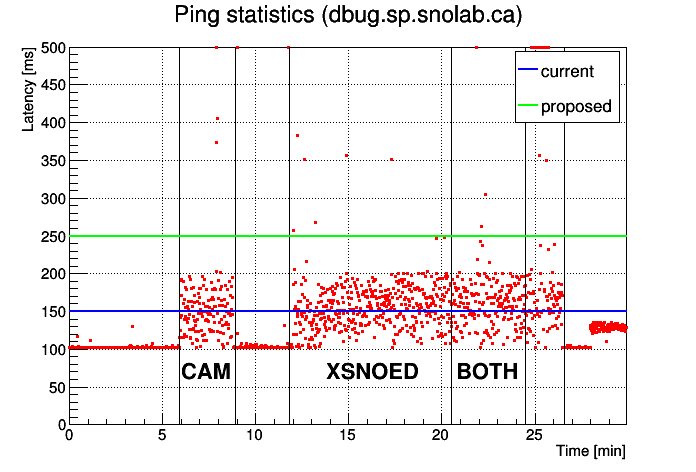
\includegraphics[width=0.8\textwidth,trim={0 3mm 0 1mm},clip]{images/dbug_martti_tests_2}
	\caption{Latency of the VPN connection on the Linux machine without any load, with the SNO+ cameras page open in Firefox (CAM), with various instances of the live event display (XSNOED), and both. The horizontal lines show the current and proposed thresholds for a timeout of the monitoring apps.}
	\label{load_linux}
\end{figure}

\begin{figure}[htp]
	\centering
	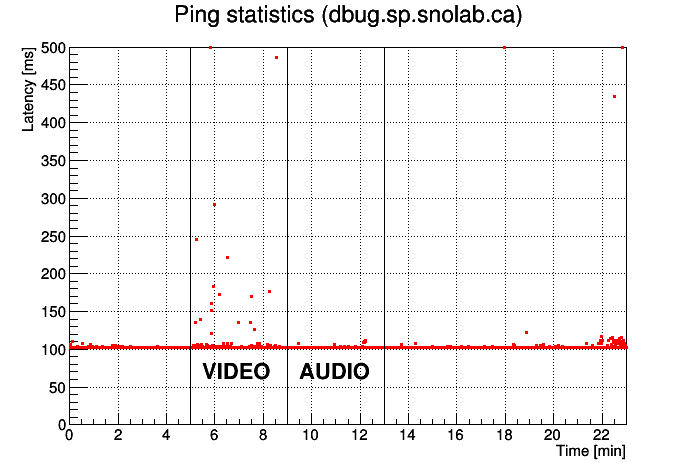
\includegraphics[width=0.8\textwidth,trim={0 3mm 0 1mm},clip]{images/dbug_martti_tests_mac}
	\caption{Latency of the VPN connection on the Mac without any load, with the TUB camera stream (VIDEO) and with the video disabled (AUDIO).}
	\label{load_mac}
\end{figure}

To fix these problems, a second monitoring machine was installed, which runs any streaming-type applications (xsnoed, cameras, etc.). The latency on this machine is now higher than usual (200~ms) but this doesn't affect the latency on other machines. Therefore, the first monitoring machines which runs the rest of monitoring applications (alarm gui, check rates gui, fec fifo, mtc gui, polling gui, daq log, builder and supernova gui) has a typical latency of 100-150~ms.

Finally, a number of hosts was pinged for 10 days straight, during which 4 shifts were taken from CRSU. Detailed results can be found in \Cref{app:latency}. It was seen that the overseas connection to the SNOLAB VPN was stable during the entire time (apart from the intermittent ping failures that all remote stations have seen), with a baseline latency of 102~ms. The fluctuations up to 200~ms are seen only for machines on the network. This suggests that the network problems are not between Europe and Canada, but rather between the SNOLAB VPN host (on surface) and the machines on the network (underground).

%%%%%%%%%%%%%%%%%%%%%%%%%%%%%%%%%%%%%%%%%%%%%%%%%%%%%%%%%%%%%%%%%%%%%%%%%%%%%%%%

\section{Communication tools}
There already was a landline phone available in the lab. We simply had it moved to the shift station desk (different port).
Because the phone was rarely used to begin with, we consider this to be a dedicated SNO+ phone.
It is possible to dial international numbers, which we tested by calling the SNOLAB control room (and picking up ourselves using the software phone).
The number for the CRSU landline is:

\qquad{\tt +44 1273 678781}

On the Windows machine (in our case a VM running on Linux), one needs to install the software phone to answer calls to the on-site control rooms (CRAG/CRUG). SNOLAB IT has put together a support page for setting up IP Communicator:

\qquad\link{https://www.snolab.ca/docushare/dsweb/View/Wiki-11/IP\%20Communicator}

It will take about one working day for them to add your device name to their system. It was possible to pick up incoming calls and also place outgoing calls to other machines on-site. It was not possible to dial external numbers using the software phone, for which we would use the landline.

The Slack application was installed on the Mac. Filling out the shift report should remind the shifters to log in, if they haven't done so already.

%%%%%%%%%%%%%%%%%%%%%%%%%%%%%%%%%%%%%%%%%%%%%%%%%%%%%%%%%%%%%%%%%%%%%%%%%%%%%%%%

\section{DAQ control and monitoring}
At times, the DAQ logger would close unexpectedly. We were able to restart {\tt tail\_daq\_log} without problems. It is unclear why this happened, but it may be related to aforementioned latency issues (timeout).

The alarm GUI intermittently showed {\tt db\_lost} alarms with a high frequency, which would clear up after a few seconds. A similar problem was reported by CROX \cite{doc5051}. This issue became very annoying as it made using the headset (e.g. for the software phone) unbearable. We noticed that the alarm GUI tries to query the database every second, and produces an alarm if the last successful query was more than 10 seconds ago. We edited the {\tt alarm\_gui} script to change the database hostname to its IP address (in case of DNS issues), and increased the alarm threshold to 20 seconds. This made the alarms a lot less frequent, as can be easily understood by studying \Cref{alarm_gui}.

After realising that these issues were caused by an increased latency, we managed to resolve the problem by running {\tt xsnoed} on a separate machine. The time since the last successful query then dropped to 2-5 seconds, and we were able to revert the above changes. After the installation of second monitoring machine there were no more reports of connection loss by the alarm GUI.

\begin{figure}[htp]
	\centering
	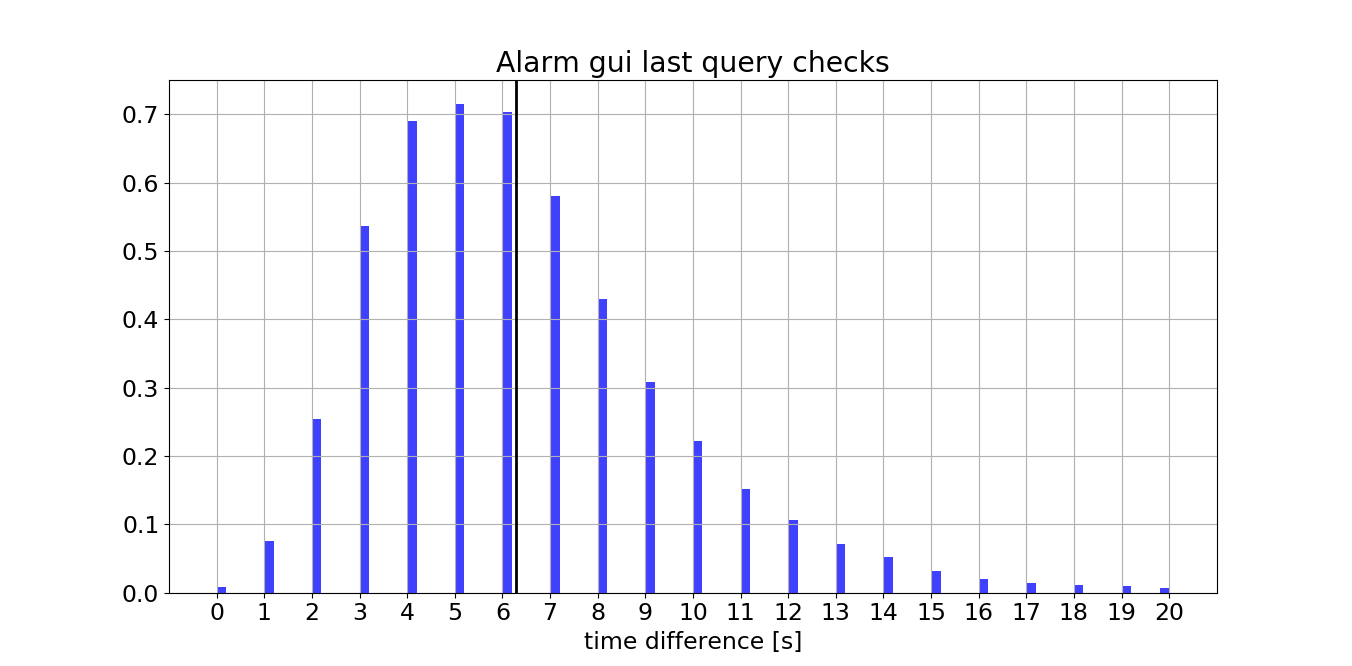
\includegraphics[width=0.8\textwidth,trim={25mm 4mm 32mm 13mm},clip]{images/alarm_gui_checks}
	\caption{Time since last successful query as registered by the alarm GUI. The average time is indicated by the black line at 6.2~s, but a significant fraction of the distribution is above 10~s.}
	\label{alarm_gui}
\end{figure}

We also ran into problems checking CMOS rates and base currents, as both the scripts would tend to crash due to timeouts. This caused another problem, which is best understood by looking at the sequence of {\tt check\_rates}:
\begin{enumerate}
	\item Set EXT2 trigger bit to high.
	\item Poll base currents / CMOS rates.
	\item Set EXT2 trigger bit to low.
	\item Evaluate polling results.
\end{enumerate}
If the script crashes in step 2, the EXT2 trigger will be left high, which will cause other problems with the detector (increased rates, possibly baseline shifts?). The {\tt check\_rates} script must be run successfully to fix this. The problem is again due to the timeout threshold being set too low. Notably, CROX reported a similar problem -- they then increased the timeout from 30~ms to 150~ms for all monitoring tools \cite{doc5051}. Based on our extensive latency tests (see \Cref{app:latency}), the timeout should perhaps be increased to 250~ms to avoid further issues of this kind.

The polling GUI could also not be run without error due to high latency. Both {\tt check\_rates} and {\tt polling\_gui} would run fine after moving the programs causing the latency increase to another machine.

To run the supernova GUI, one needs to obtain the significance file periodically from the KamLAND server. Access to that server may be requested (for 1 machine per institution/group only) using the following web form (thanks to Matt Strait for pointing this out):

\qquad\link{http://www.awa.tohoku.ac.jp/kamland/SNmonitor/regist/cgi-bin/regist.py}

In most cases, KamLAND colleagues will then add the requested IP address within a week.
Another option is to run the app from monag1 via {\tt ssh}.

%%%%%%%%%%%%%%%%%%%%%%%%%%%%%%%%%%%%%%%%%%%%%%%%%%%%%%%%%%%%%%%%%%%%%%%%%%%%%%%%

\section{ORCA control and functionality}
During the shadow shifts, we tested a number of ORCA handovers: The ``old'' shifter would save ORCA and let the ``new'' shifter know when this was done. At CRSU, saving ORCA would take about 30~seconds. The new shifter would then check the mounted shared volume to see when the ORCA file ({\tt snot\_main.orca}) was last modified. If the time shown was within 2~minutes of the current time, the new shifter would start ORCA (having made sure the correct version was installed). Once ORCA was up, the ``could not obtain lock'' alert would be displayed. The old shifter was then informed of this (``waiting for lock'') and closed their version of ORCA. This would result in a lock being obtained within 10~seconds, at which point the new shifter has detector control. It is important that the new shifter remembers to take control of the alarm GUI (operator mode) and the scope as soon as possible.

While it was possible to restart a run within a reasonable amount of time, we found that we could not resync a run when this became necessary. ORCA would start a new run, during which this error message would come up in the builder:

{\footnotesize
\begin{Verbatim}[xleftmargin=-8mm]
	20180421 14:18:57 WR.6: Inserted RHDR record for GT 000001 before 000001 in header queue
	20180421 14:18:57 WR.2: Error: No output file open! -- opening default file.
	20180421 14:18:57 WR.2: WARNING: Pmt event records will NOT have correct run/subrun numbers
	20180421 14:18:57 WR.2: **** Start a new run IMMEDIATELY to fix this!!!! ****
	20180421 14:18:57 WR.0: Created output zdab file default_000759.zdab
\end{Verbatim}
}

While it was sometimes possible (see below) to restart a run after that, it was unclear whether a full resync had occurred. Therefore, we could not consider this a successful resync. Typically, detector control was then handed over to CRAG for a resync. The same issue was later also observed when switching from a Maintenance run to a Physics run. However, restarting the run would resolve the issue.

More problematically, ORCA would frequently crash. Sometimes this happened randomly, but more often it was just after starting ORCA or while trying to do something (e.g. restart/resync run). The crash logs mostly reported the same uncaught exception:

{\footnotesize
\begin{Verbatim}[xleftmargin=-8mm]
	22 Exception Type:        EXC_BAD_INSTRUCTION (SIGILL)
	23 Exception Codes:       0x0000000000000001, 0x0000000000000000
	24 Exception Note:        EXC_CORPSE_NOTIFY
	25 
	26 Termination Signal:    Illegal instruction: 4
	27 Termination Reason:    Namespace SIGNAL, Code 0x4
	28 Terminating Process:   exc handler [0]
	29 
	30 Application Specific Information:
	31 *** Terminating app due to uncaught exception 'NSGenericException', 
	   reason: '-[NSAlert runModal] may only be invoked from the main thread.
	   Behavior on other threads is undefined.
\end{Verbatim}
}

It was clear that these problems had to be resolved before CRSU can be approved for autonomous shifting. After intense debugging all the known issues were fixed, the process is described in \Cref{app:ORCA}.

%%%%%%%%%%%%%%%%%%%%%%%%%%%%%%%%%%%%%%%%%%%%%%%%%%%%%%%%%%%%%%%%%%%%%%%%%%%%%%%%

\section{Issues}
We discussed the aforementioned issues on the DAQ call on 25/04/2018:
\begin{itemize}
	\item To better understand the ORCA crashes, it was suggested that we connect to the test stand from CRSU and attempt to reproduce the unexpected ORCA behaviour, as this may provide valuable information for debugging. The teststand timing rack was powered on on 27/04/2018 and the ORCA crash was successfully reproduced. Looking at the ORCA code, {\tt runModal} is only called twice in the main ORCA function: Once to check that the correct version is running, and once to verify that the running version has a lock on the shared ORCA file. The latter check is run once every 5 seconds, and is only expected to run when starting ORCA. This issue was later fixed, the details are included in \Cref{app:ORCA}.
	
	\item Regarding the latency issues, we were advised to discuss matters again with ITS. They offered for us to run tests in the Shawcross building, which hosts the data centre and would allow us to circumvent the old Pevensey~II network. However, despite being much closer to the central network and having access to a 1~Gbps internet connection, the latency did not improve. This led us to the hypothesis that the problem lies between the SNOLAB VPN host (on surface) and the individual machines on the network (underground).
	
	Additionally, we wrote a script to continuously ping a host, printing a Unix timestamp (seconds since 01/01/1970) and the current latency (milliseconds) to screen. The script was successfully tested on various flavours of Linux (Ubuntu, CentOS, Scientific) and Mac OSX (Darwin), and was then added to Karin's remote monitoring tools:

	\qquad\link{https://github.com/snoplus/remote-network-monitor}
	
	We suggest that other overseas remote control rooms (CROX, CRLIP) test this script to determime whether they see a similar increase in latency when connected to ``streaming'' applications like {\tt xsnoed} or various cameras at SNOLAB.
\end{itemize}

%%%%%%%%%%%%%%%%%%%%%%%%%%%%%%%%%%%%%%%%%%%%%%%%%%%%%%%%%%%%%%%%%%%%%%%%%%%%%%%%

\section{Conclusions and summary}
A remote shift station was commissioned at the University of Sussex.
A number of issues were encountered, all of which have now been resolved.
They can be grouped into two categories: issues caused by high latency, and ORCA crashes.
The issues caused by high latency were partially resolved by setting up a second monitoring machine in the control room.
Additionally, Sussex ITS had to disable all the local firewalls and network monitoring tools for the SNOLAB VPN address and ports.
ORCA crashes have now been resolved, as detailed in \Cref{app:ORCA}.
A total of 4 shadow shifts and 10 independent shifts have now been taken from CRSU, with increasingly stable conditions.
It would be useful if shifters could run the advanced set of network monitoring tools at other remote control rooms, especially at other overseas institutions.

%%%%%%%%%%%%%%%%%%%%%%%%%%%%%%%%%%%%%%%%%%%%%%%%%%%%%%%%%%%%%%%%%%%%%%%%%%%%%%%%

\begin{thebibliography}{99}
\bibitem{doc4428}
T.~LaTorre, \docdb{4428}

\bibitem{doc4776}
A.~Mastbaum, E.~Caden, T.~LaTorre and E.~Leming, \docdb{4776}

\bibitem{doc5040}
K.~Gilje and J.~P.~Y\'{a}\~{n}ez-Garza, \docdb{5040}

\bibitem{doc5051}
E.~Leming, \docdb{5051}
\end{thebibliography}

%%%%%%%%%%%%%%%%%%%%%%%%%%%%%%%%%%%%%%%%%%%%%%%%%%%%%%%%%%%%%%%%%%%%%%%%%%%%%%%%

\appendix
\section{Appendix}

% After our extremely thorough tests, we don't really need the first section any more.

% \subsection{Network connectivity plots\label{app:network}}
% 
% \Cref{internet_linux,internet_mac,vpn_linux,vpn_mac} show the network connectivity plots produced using Karin's scripts \cite{doc5040}.
% 
% \begin{figure}[htp]
% 	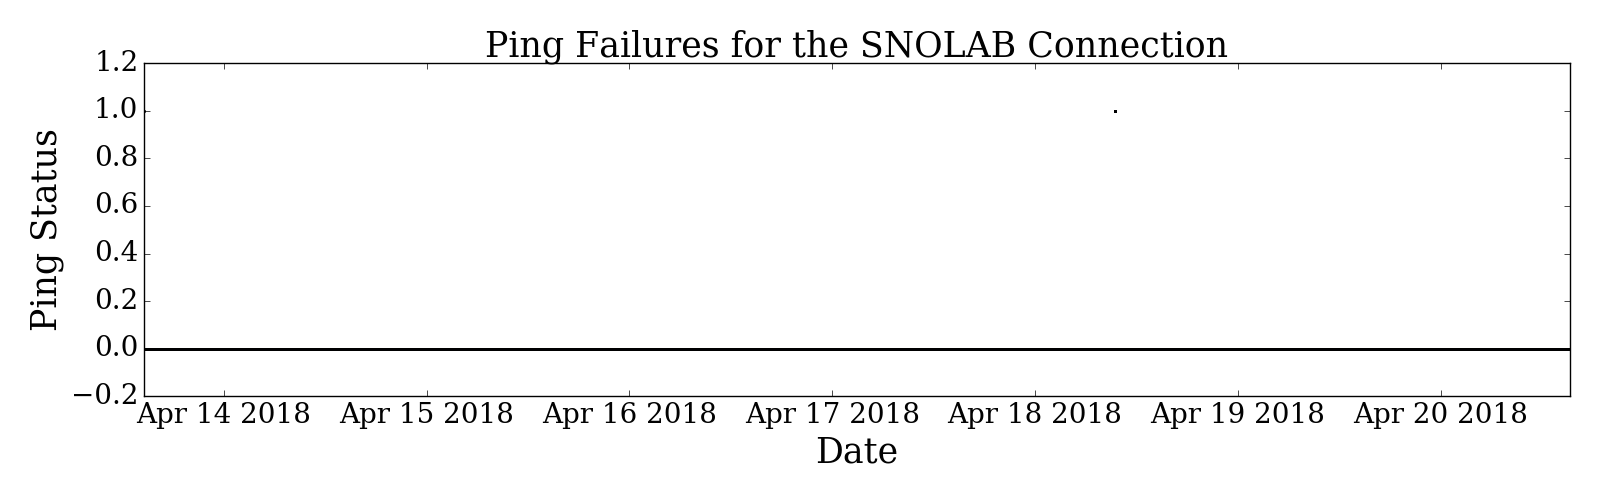
\includegraphics[width=\textwidth,trim={5mm 7mm 5mm 5mm},clip]{images/SNOLAB_ping_failures.png}
% 	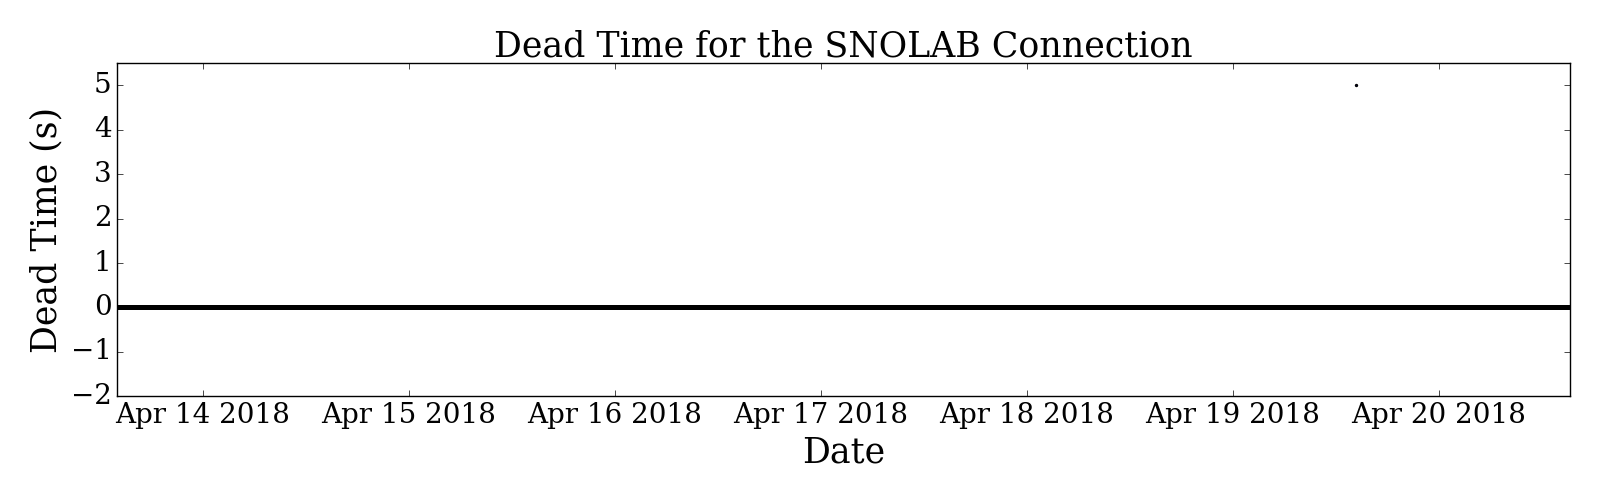
\includegraphics[width=\textwidth,trim={5mm 7mm 5mm 5mm},clip]{images/SNOLAB_dead_time.png}
% 	\caption{Internet connectivity on the Linux machine, monitored over the course of 7 days. A single failure that lasted 5 seconds was registered, caused by ITS rerouting an ethernet cable.}
% 	\label{internet_linux}
% \end{figure}
% 
% \begin{figure}[htp]
% 	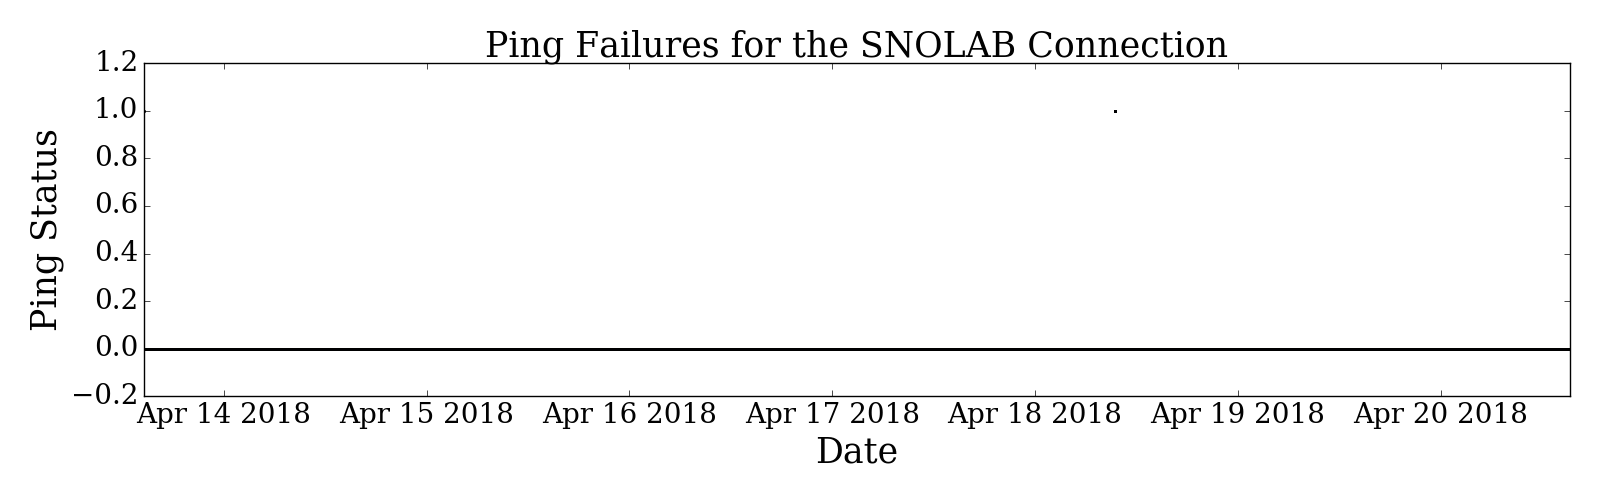
\includegraphics[width=\textwidth,trim={5mm 7mm 5mm 5mm},clip]{images/SNOLAB_ping_failures.png}
% 	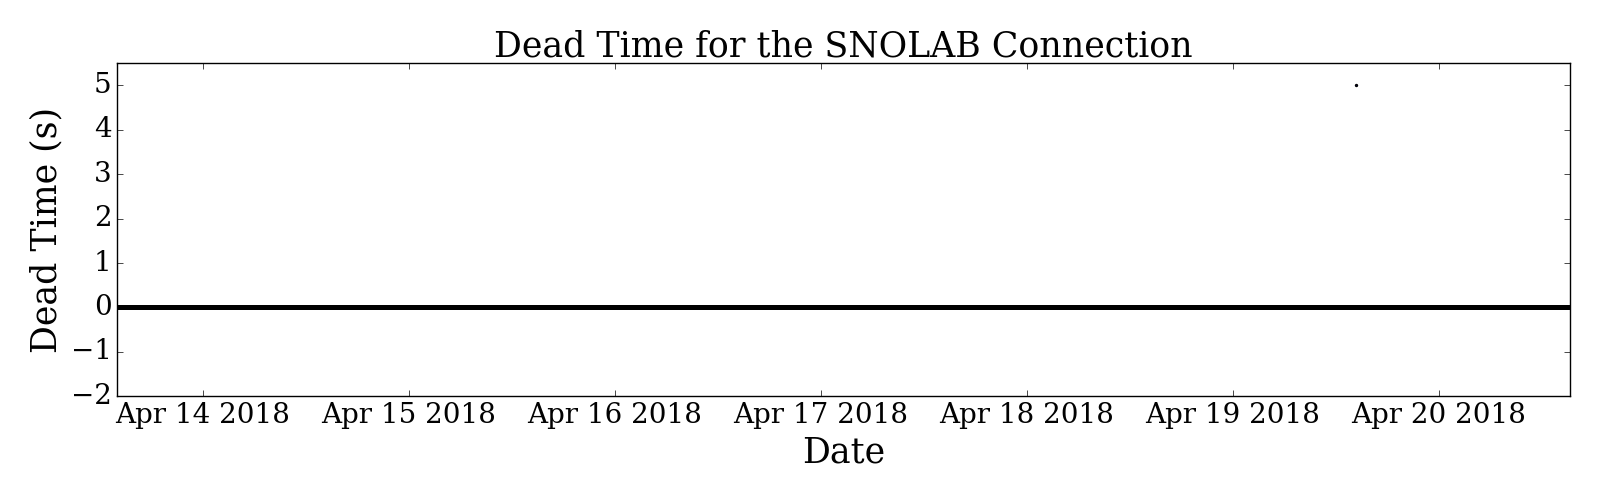
\includegraphics[width=\textwidth,trim={5mm 7mm 5mm 5mm},clip]{images/SNOLAB_dead_time.png}
% 	\caption{Internet connectivity on the Mac machine, monitored over the course of 7 days. A single failure that lasted 70 seconds was registered, corresponding to the time an IT expert was rerouting our ethernet socket (i.e. the ethernet cable was unplugged).}
% 	\label{internet_mac}
% \end{figure}
% 
% \begin{figure}[htp]
% 	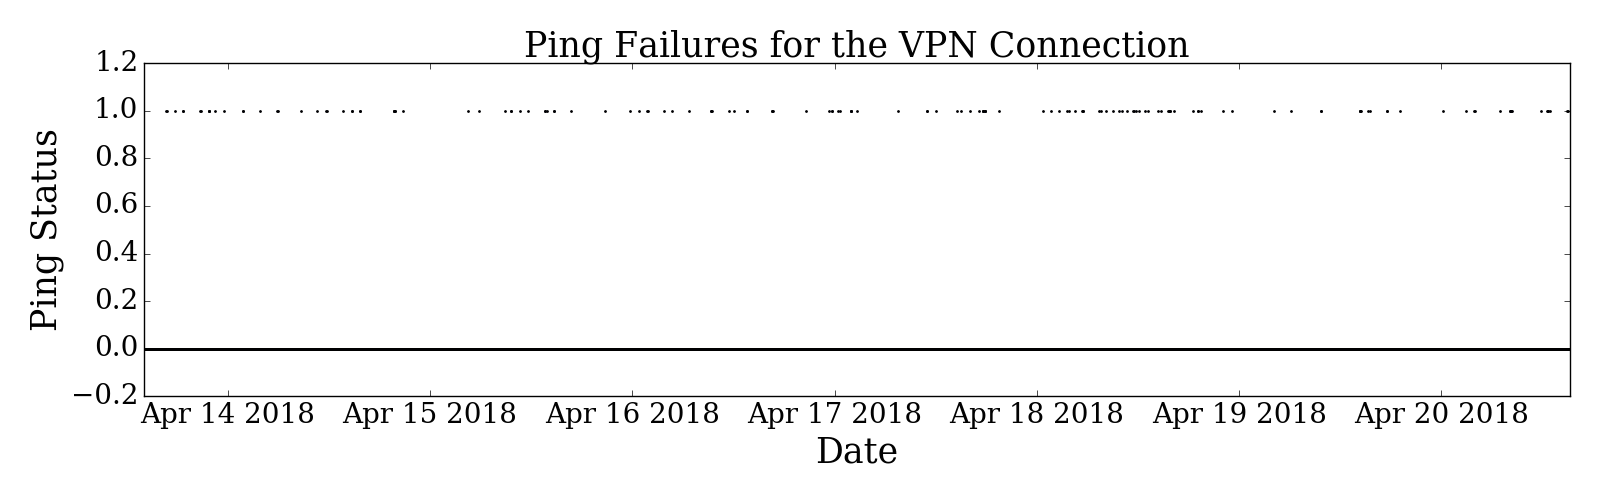
\includegraphics[width=\textwidth,trim={5mm 7mm 5mm 5mm},clip]{images/VPN_ping_failures.png}
% 	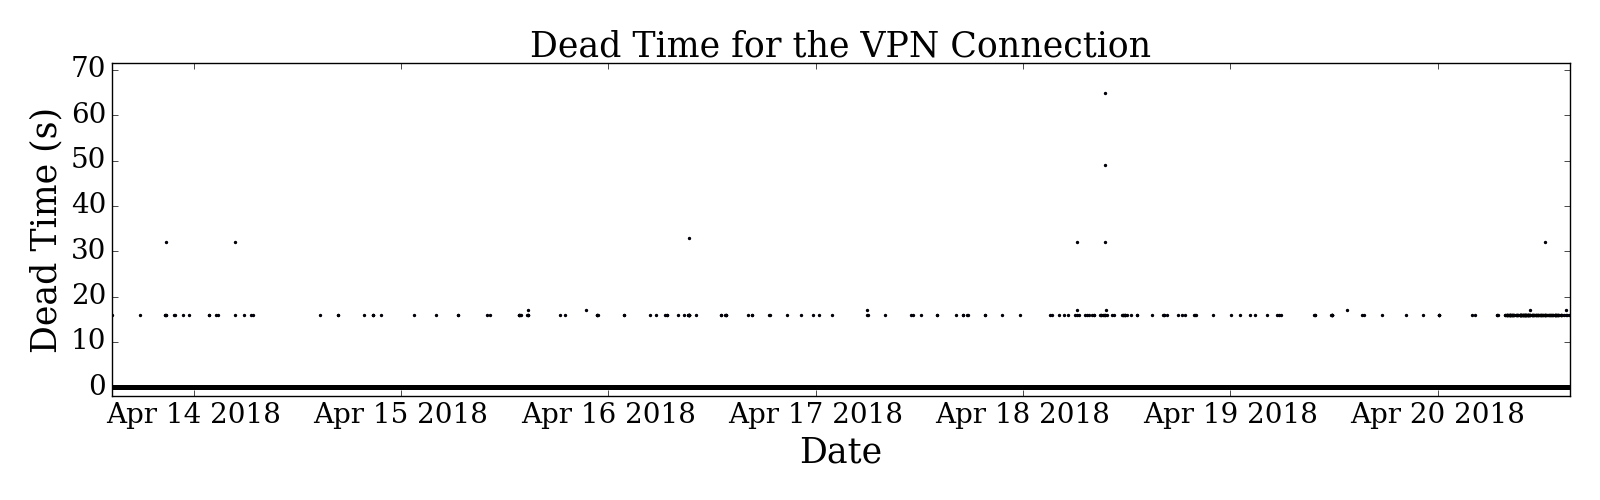
\includegraphics[width=\textwidth,trim={5mm 7mm 5mm 5mm},clip]{images/VPN_dead_time.png}
% 	\caption{VPN connectivity on the Linux machine, monitored over the course of 7 days. Ping failures occurred relatively frequently, but never lasted for longer than 30 seconds.}
% 	\label{vpn_linux}
% \end{figure}
% 
% \begin{figure}[htp]
% 	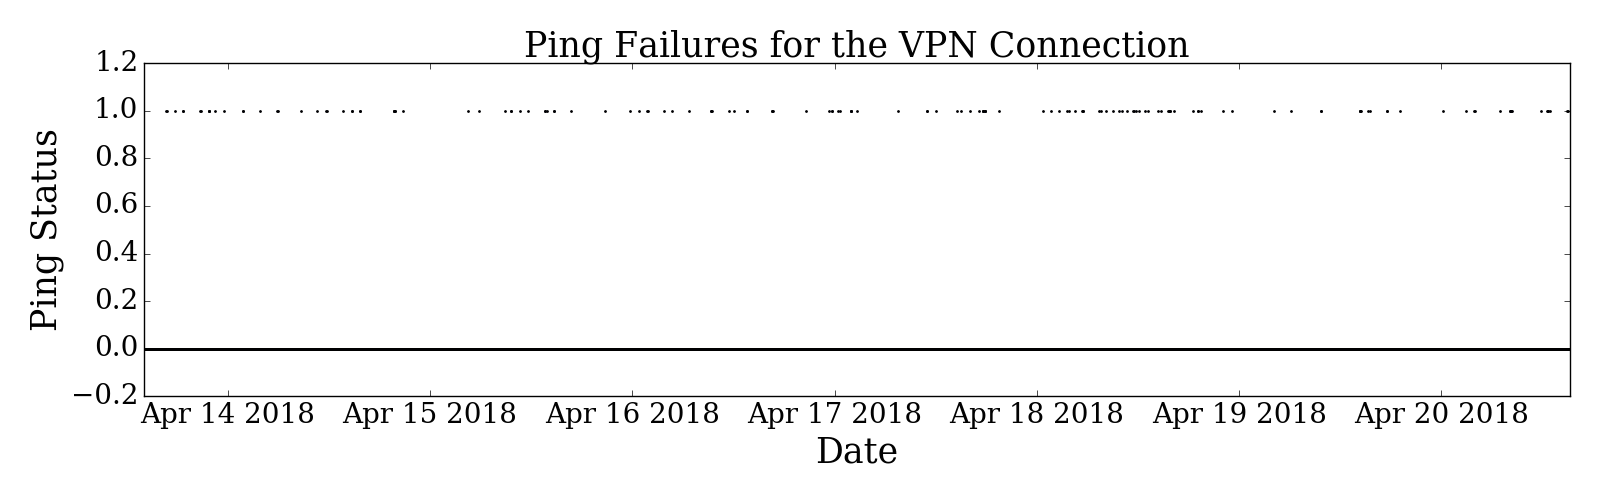
\includegraphics[width=\textwidth,trim={5mm 7mm 5mm 5mm},clip]{images/VPN_ping_failures.png}
% 	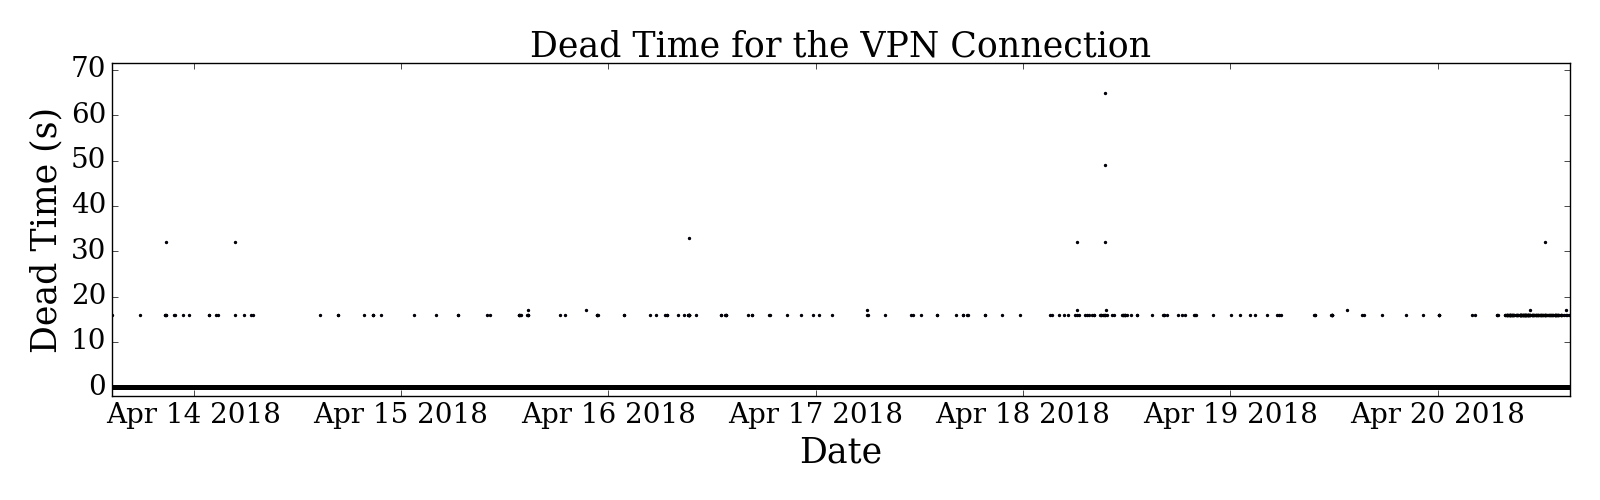
\includegraphics[width=\textwidth,trim={5mm 7mm 5mm 5mm},clip]{images/VPN_dead_time.png}
% 	\caption{Same as Fig.~\ref{vpn_linux}, but for the Mac. The 70~second disconnect corresponds to the ethernet cable being swapped, see Fig.~\ref{internet_mac}.}
% 	\label{vpn_mac}
% \end{figure}

% \clearpage
\subsection{Latency plots\label{app:latency}}

% \Cref{ping_linux,ping_mac} show the latency over time, where the on-site machine {\tt buffer1.sp.snolab.ca} was being pinged. The latency was monitored from Monday to Friday until the end of the first shadow shift.

% \Cref{no_load_linux,no_load_mac} show the latency monitored over 25 hours for the Linux and Mac machines, respectively. Neither machine was running any software other than the VPN during that time, and the on-site machine {\tt dbug.sp.snolab.ca} was being pinged.

% Lastly, histograms of latency to dbug after installing second monitoring machine are shown to confirm that the high latency issues were fixed.

% \begin{figure}[htp]
% 	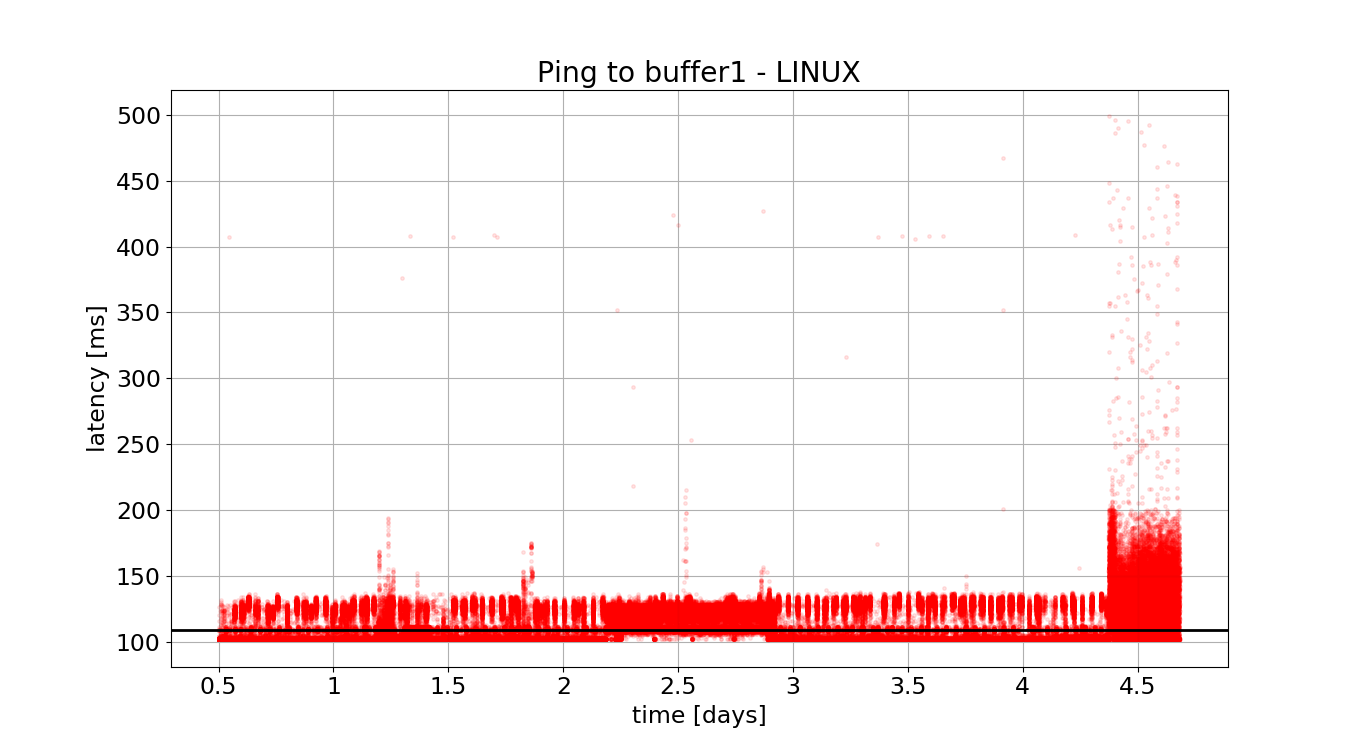
\includegraphics[width=\textwidth,trim={15mm 5mm 15mm 10mm},clip]{\string~/Dropbox/CRSU/Network/ping_plots/linux_500.png}
% 	\caption{Latency of the VPN connection on the Linux machine, monitored by pinging {\tt buffer1} over the course of 5 working days (Mon-Fri). The black line represents the global average. A cutoff is applied at 500 ms so as not to include the spikes due to the VPN reconnecting. The final phase around 4.5 days corresponds to the first CRSU shadow shift (detector was at LV).}
% 	\label{ping_linux}
% \end{figure}
% 
% \begin{figure}[htp]
% 	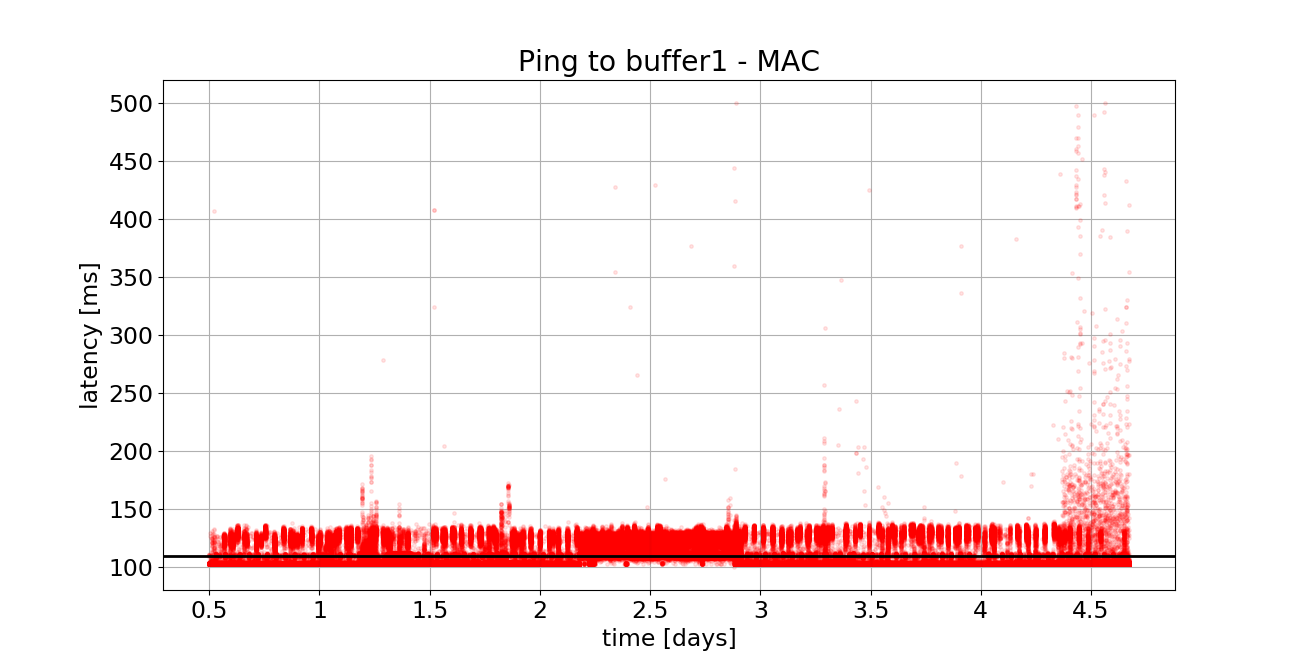
\includegraphics[width=\textwidth,trim={15mm 3mm 15mm 10mm},clip]{\string~/Dropbox/CRSU/Network/ping_plots/mac_500.png}
% 	\caption{Same as Fig.~\ref{ping_linux}, but for the Mac.}
% 	\label{ping_mac}
% \end{figure}
% 
% \begin{figure}[htp]
% 	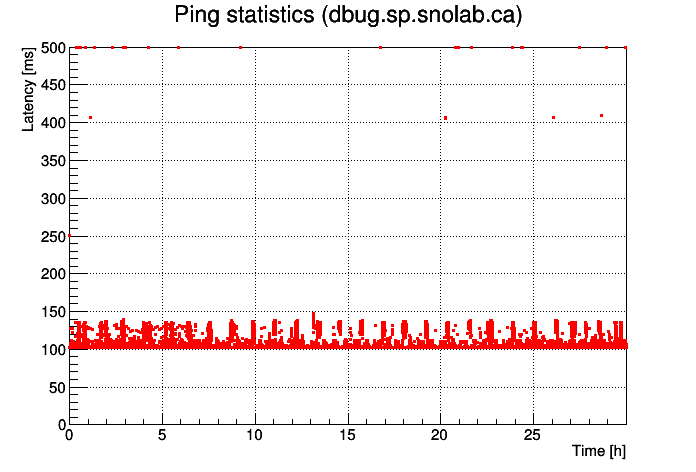
\includegraphics[width=\textwidth,trim={0 3mm 0 1mm},clip]{images/dbug_no_load_linux.pdf}
% 	\caption{Latency of the VPN connection on the Linux machine without any load, monitored over the course of a day. A cutoff is applied at 500~ms, any higher values (or timeouts) are set to that value. There are periodic increases to around 130~ms about once an hour, which we assume to be due to increased on-site activity (e.g. copying of files after a run rollover).}
% 	\label{no_load_linux}
% \end{figure}
% 
% \begin{figure}[htp]
% 	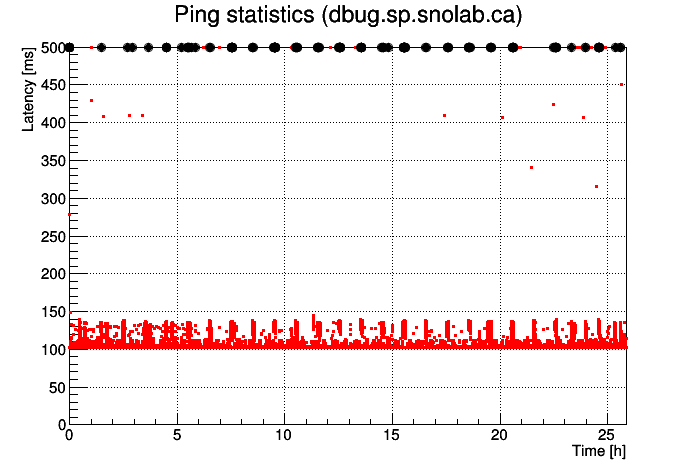
\includegraphics[width=\textwidth,trim={0 3mm 0 1mm},clip]{images/dbug_no_load_mac.pdf}
% 	\caption{Same as \Cref{no_load_linux}, but for the Mac. The large black dots indicate ping timeouts. It is unclear what caused these, as the Linux machine did not see any timeouts.}
% 	\label{no_load_mac}
% \end{figure}

% Histograms removed, as they aren't really useful in this context
% \begin{figure}[htp]
% 	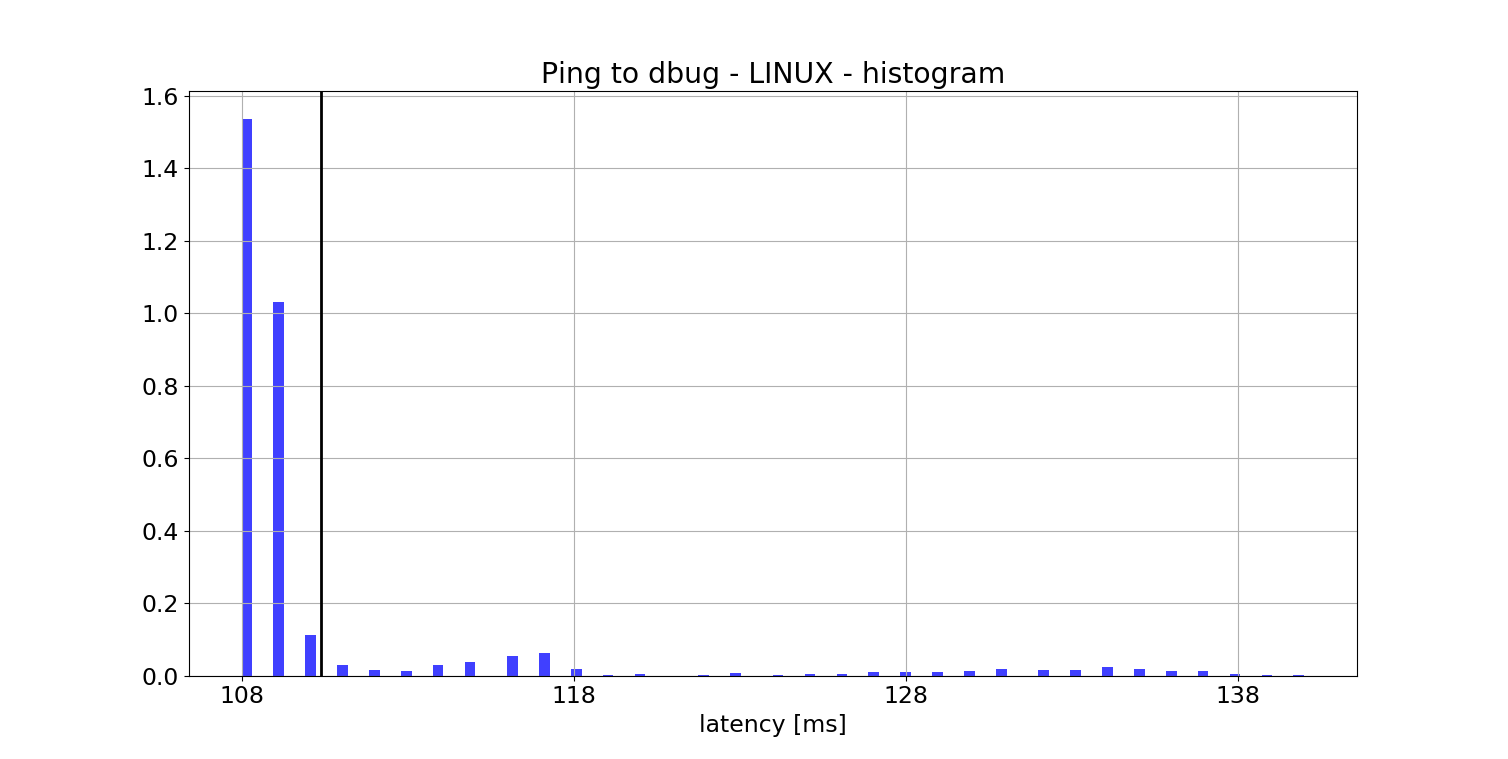
\includegraphics[width=\textwidth,trim={0 0 0 0},clip]{\string~/Dropbox/CRSU/Network/no_load/no_load_linux_hist.png}
% 	\caption{Histogram of latency of the connection to dbug on the linux, after having 2 monitoring machines installed. The vertical line represents the average. The data was taken for period of many days.}
% 	\label{linux_hist_final}
% \end{figure}
% 
% \begin{figure}[htp]
% 	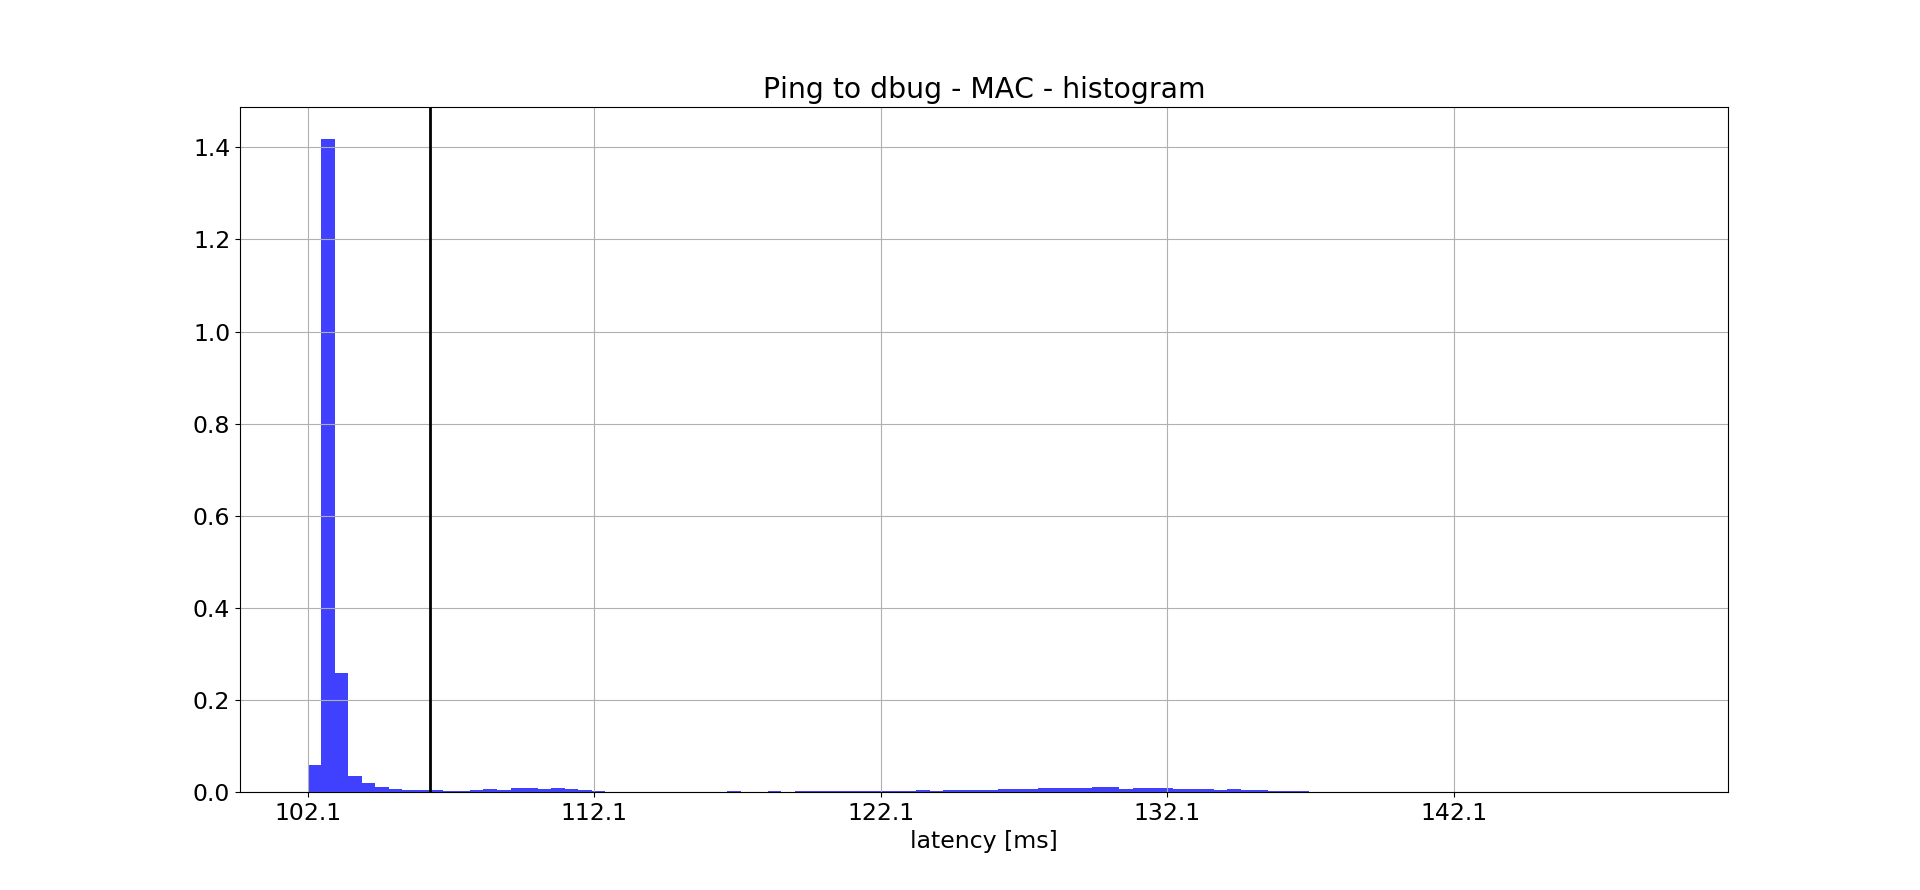
\includegraphics[width=\textwidth,trim={0 0 0 0},clip]{\string~/Dropbox/CRSU/Network/no_load/no_load_mac_hist.png}
% 	\caption{Histogram of latency of the connection to dbug on the mac, after having 2 monitoring machines installed. The vertical line represents the average. The data was taken for period of many days.}
% 	\label{mac_hist_final}
% \end{figure}

The most comprehensive latency tests were run by Martti from 25/05/2018 -- 05/06/2018, for an uninterrupted duration of over 10 days. From each machine (monsu1, monsu2, opersu) the following hosts were pinged continuously, with a pause of 1 second in between pings:
\begin{Verbatim}
	www.oxford.ac.uk
	vpn1.snolab.ca
	buffer1.sp.snolab.ca
	dbug.sp.snolab.ca
\end{Verbatim}
While the first two are reachable globally, the latter two machines can only be pinged while connected to the VPN.
Oxford University was pinged to determine that the internet connection at Sussex was up and running, and to check that there are no latency problems within the UK.
SNOLAB VPN was pinged to demonstrate the availability of the VPN, and that the latency is stable here. This was indeed the case, with minimal ping values just above 100~ms being seen throughout.
\Cref{latency_final_1,latency_final_2,latency_final_3} show the results of these tests.

\begin{figure}[htp]
	\centering
	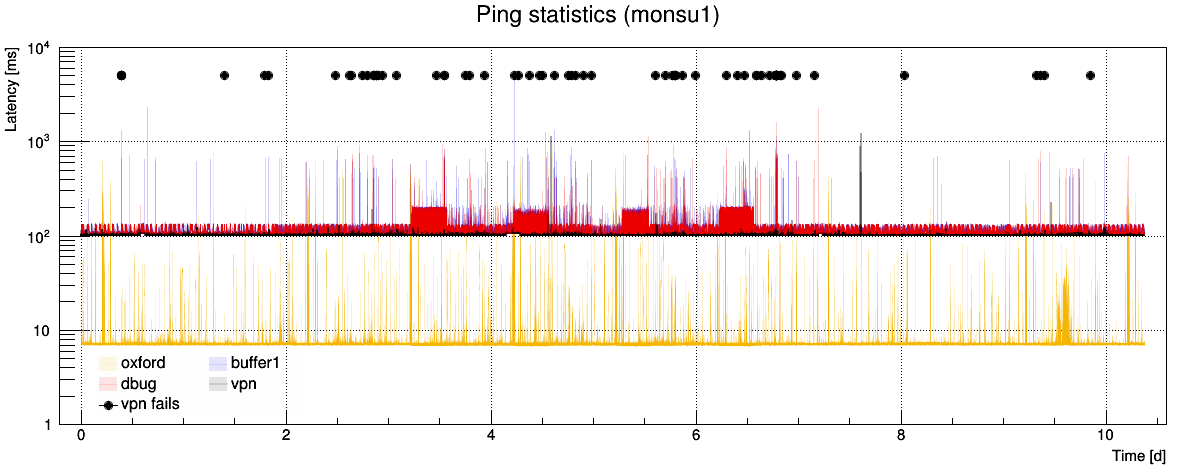
\includegraphics[width=\textwidth]{images/monsu1_latency}\\
	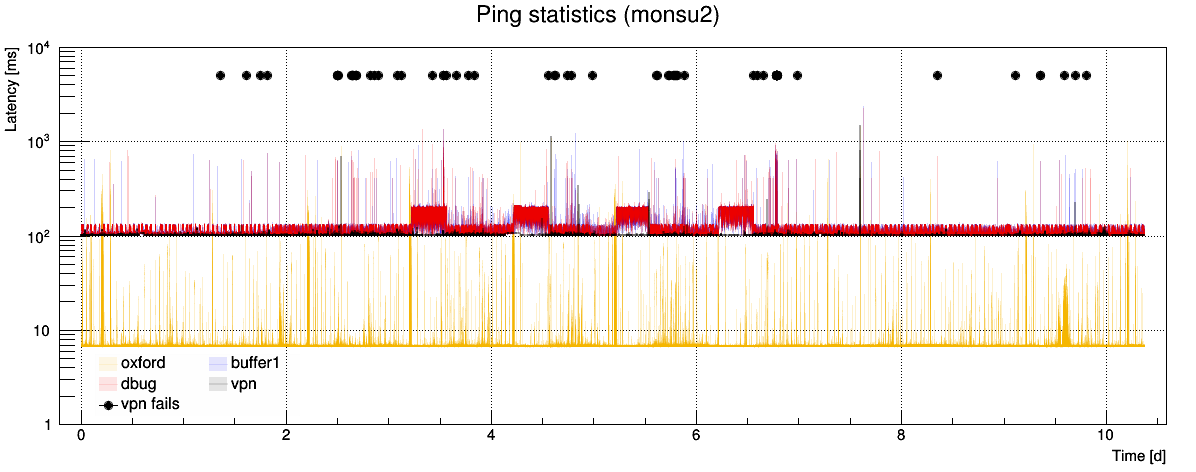
\includegraphics[width=\textwidth]{images/monsu2_latency}\\
	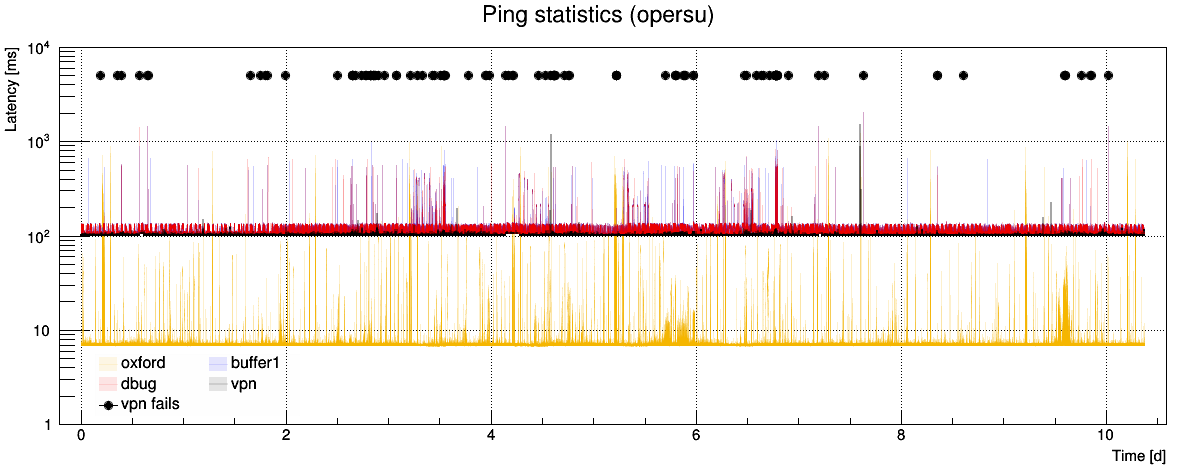
\includegraphics[width=\textwidth]{images/opersu_latency}
	\caption{Various latencies at CRSU, monitored continuously over the course of 10 days. Note the logarithmic vertical scale. The latency to the UK host is of the order of 10~ms, while the latency to overseas machines tends to be of the order of 100~ms. VPN disconnects are represented by black dots, set to an arbitrary value of 5~s.}
	\label{latency_final_1}
\end{figure}

\begin{figure}[htp]
	\centering
	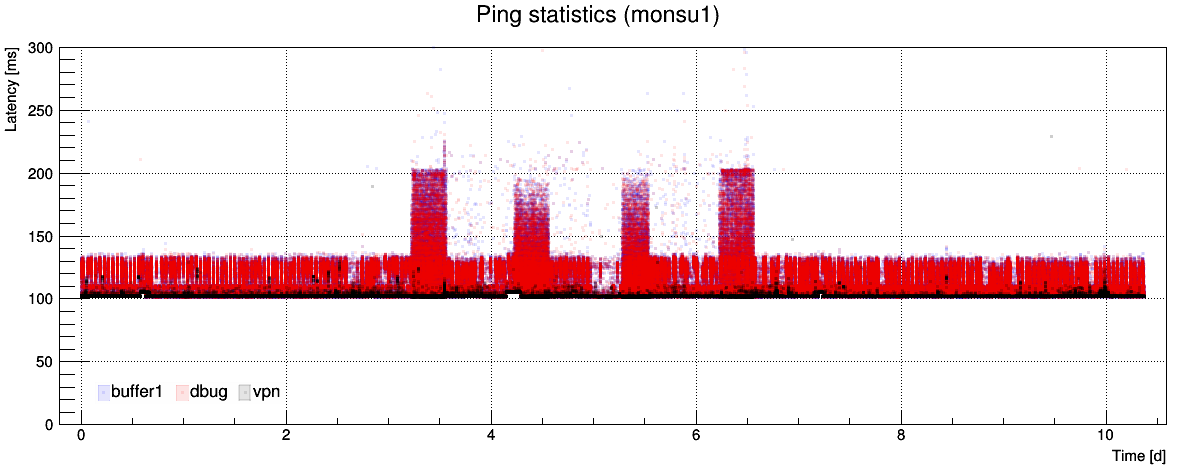
\includegraphics[width=\textwidth]{images/monsu1_latency_zoom}\\
	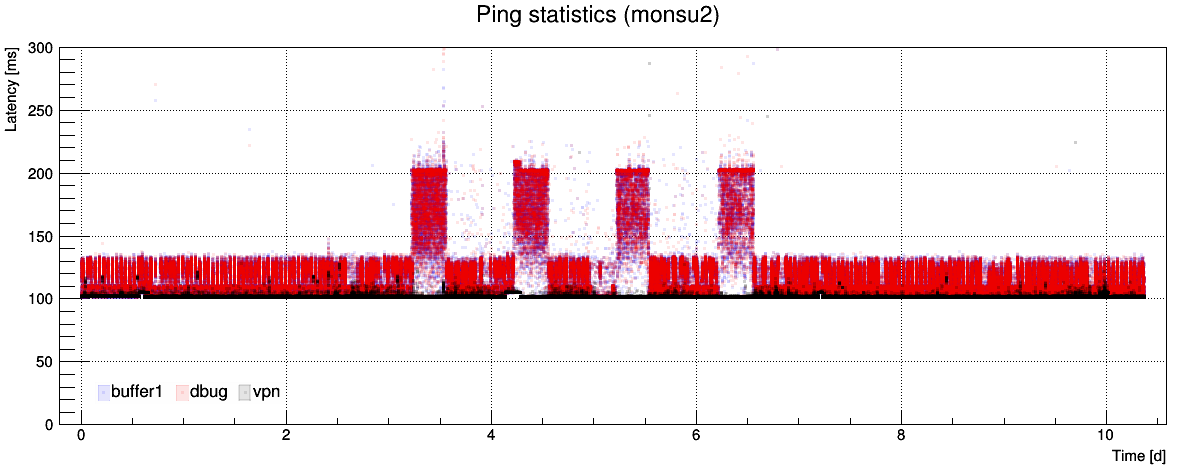
\includegraphics[width=\textwidth]{images/monsu2_latency_zoom}\\
	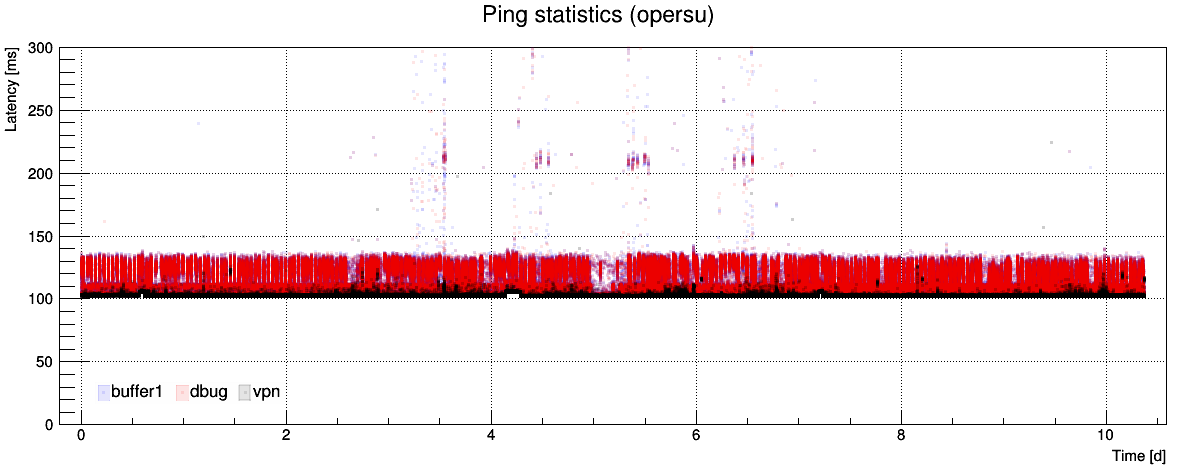
\includegraphics[width=\textwidth]{images/opersu_latency_zoom}
	\caption{Same as \Cref{latency_final_1}, but showing only the latencies for SNOLAB hosts, as a scatterplot on a linear scale. It can clearly be seen when CRSU was running under load, i.e. taking shifts (graveyard shifts 28/05/2018 -- 31/05/2018). The VPN connection (black dots) however remains stable at a relatively low 102~ms.}
	\label{latency_final_2}
\end{figure}

\begin{figure}[htp]
	\centering
	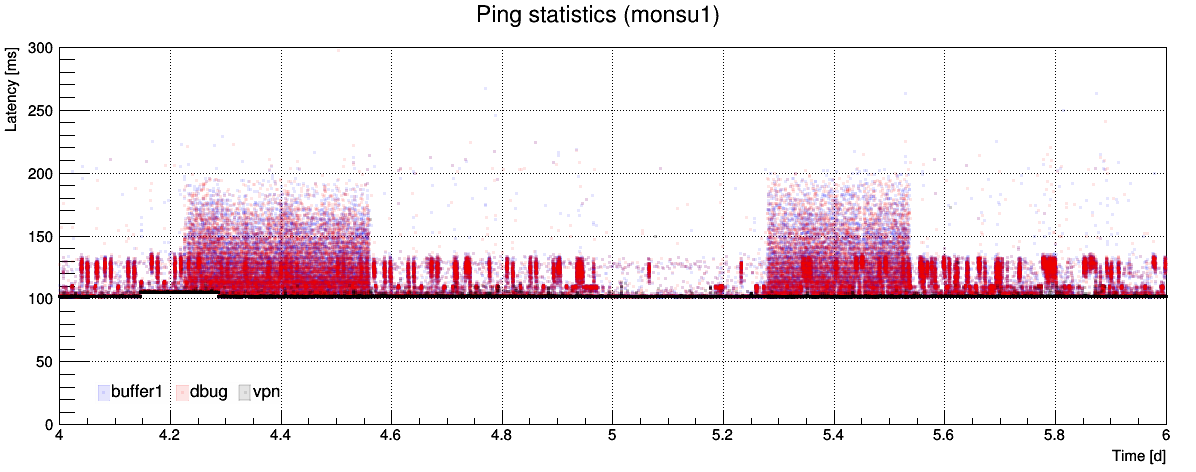
\includegraphics[width=\textwidth]{images//monsu1_latency_zoom_shift}\\
	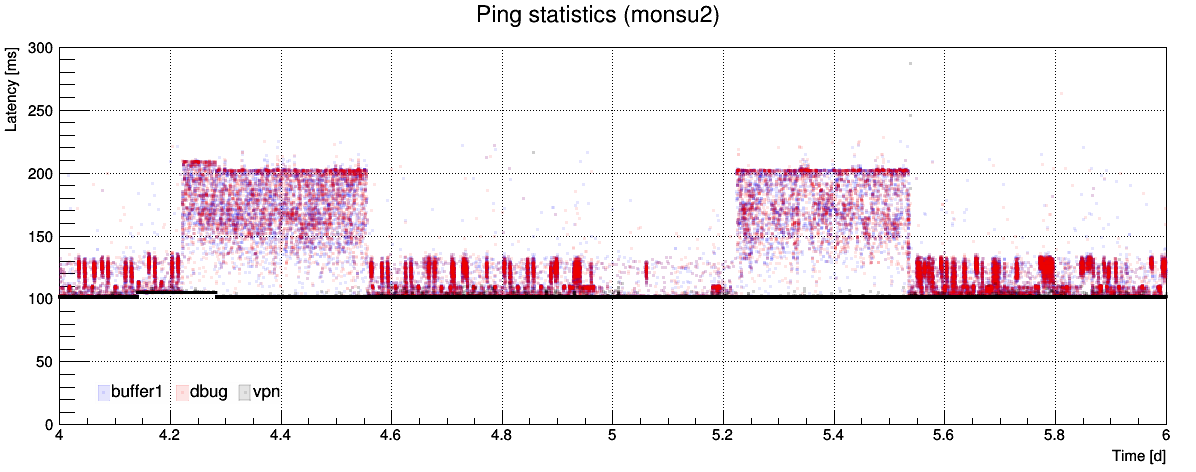
\includegraphics[width=\textwidth]{images//monsu2_latency_zoom_shift}\\
	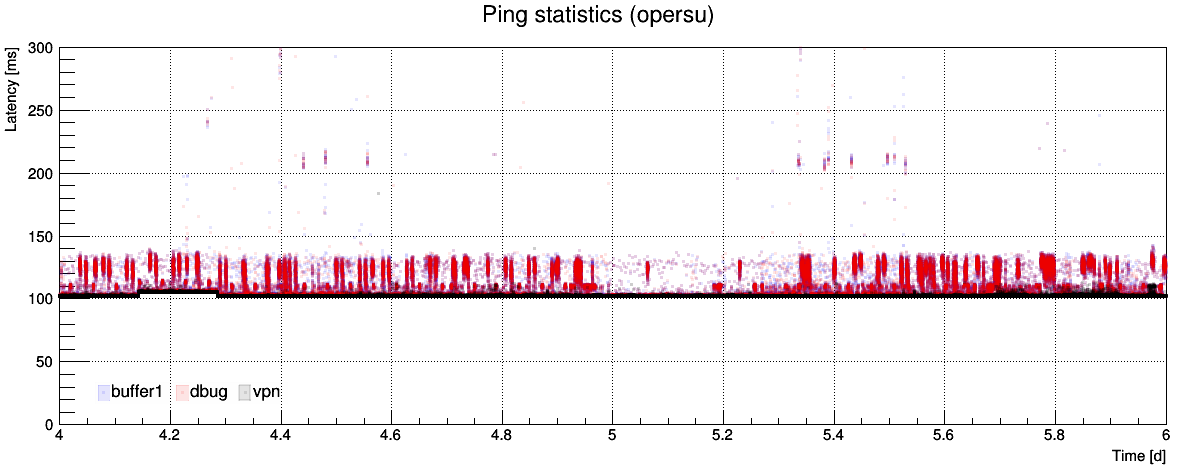
\includegraphics[width=\textwidth]{images//opersu_latency_zoom_shift}
	\caption{Same as \Cref{latency_final_2}, but zoomed in on two of the days during which shifts were being taken at CRSU. On monsu1, which runs most monitoring tools as well as the software phone, the typical latency was just above 100~ms, with occasional fluctuations up to 200~ms. On monsu2 however, which monitored the cameras as well as 4 instances of xsnoed, the latency was most often at its highest values, i.e. 200~ms. The operating machine, which runs ORCA and the TUBii audio, was least affected by the latency fluctuations. The occasional peaks around 210~ms may be due to saving the ORCA file.}
	\label{latency_final_3}
\end{figure}


\clearpage
\subsection{ORCA crashes\label{app:ORCA}}
\paragraph{TUBiiModel - restartKeepAlive}
The very first issue encountered was issue with a check for TUBii state. The modal dialogue ({\tt [NSAlert runModal]}) was called from non-main thread. This caused ORCA to crash at start and/or sometimes at random times while running. This was fixed by Ed's PR 504, which forces the offensive method to call onto the main thread:

\qquad\link{https://github.com/snoplus/orca/pull/504}. 

\paragraph{Assertion failures}
There were several assertion failures caused by ORCA. The most severe one was encountered when trying to store to a local file (i.e. saving ORCA settings):
\begin{Verbatim}[xleftmargin=-8mm]
	Assertion failure in -[NSCustomImageRep encodeWithCoder:]
\end{Verbatim}

The solution was to turn off the Foundation Assertions in the Xcode, then comment out line 44 in {\tt ORLineMarker.m}:
\begin{Verbatim}[xleftmargin=-8mm]
	[super encodeWithCoder:encoder];
\end{Verbatim}
and store afterwards. This has fixed the issue which is believed to be caused by loading an old configuration that is missing a new object. After saving the setting in this manner once the changes were reverted and all following saves worked without any issue. Mark Howe believes this should be a permanent fix. 

Other types of assertion failures were encountered when closing some of the ORCA windows, specifically the FEC view windows as well as Crate view windows. The associated error was:
\begin{Verbatim}[xleftmargin=-8mm]
	[NSTextFieldCell \_objectValue:forString:errorDescription:],
\end{Verbatim}
and similar. This was found to be happening due to empty string being passed. A simple fix of type:
\begin{Verbatim}[xleftmargin=-8mm]
	- (NSString*) comments
	  {
	    if(!comments) {return @"";}
	    else {return comments;}
	  }
\end{Verbatim}
was implemented at {\tt ORFec32.Controller.m} file (2 places) and at {\tt ORSNOCrateController.m} (1 place). It is important to note that the errors encountered when closing windows were only observed in Xcode console output and not in the ORCA log. They also didn't cause a crash, whereas the previous issues had done.

Afterwards ORCA was tested while connected to teststand. {\tt Couchdb} at teststand was modified temporarily to be accessible from the vpn. This can be done be modifying specific {\tt .ini} file. This still require VPN access so it is secure and safe as the teststand's {\tt couchdb} is not the one that the detector is connected to. We were able to start, stop, restart and resync runs without any issues. Opening and closing windows as well as saving the settings all went successfully.

For more details regarding network monitoring and ORCA issues please contact the CRSU experts.

%%%%%%%%%%%%%%%%%%%%%%%%%%%%%%%%%%%%%%%%%%%%%%%%%%%%%%%%%%%%%%%%%%%%%%%%%%%%%%%%

\end{document}
